
\subsubsection{5.1 Main Result: Graph SSL Outperforms SANE on ViT Zoo (RQ1)}

Table 1 and Figure 1 present the primary comparison. EquiSSL-perm achieves $R^{2}=0.231$ on 53 held-out ViT-S/16 models; SANE achieves $R^{2}=0.072$; EquiSSL achieves $R^{2}=0.210$. Exact values from the experiment record are: SANE 0.07215, EquiSSL 0.20981, EquiSSL-perm 0.23050.

\begin{figure}[htbp]
\centering
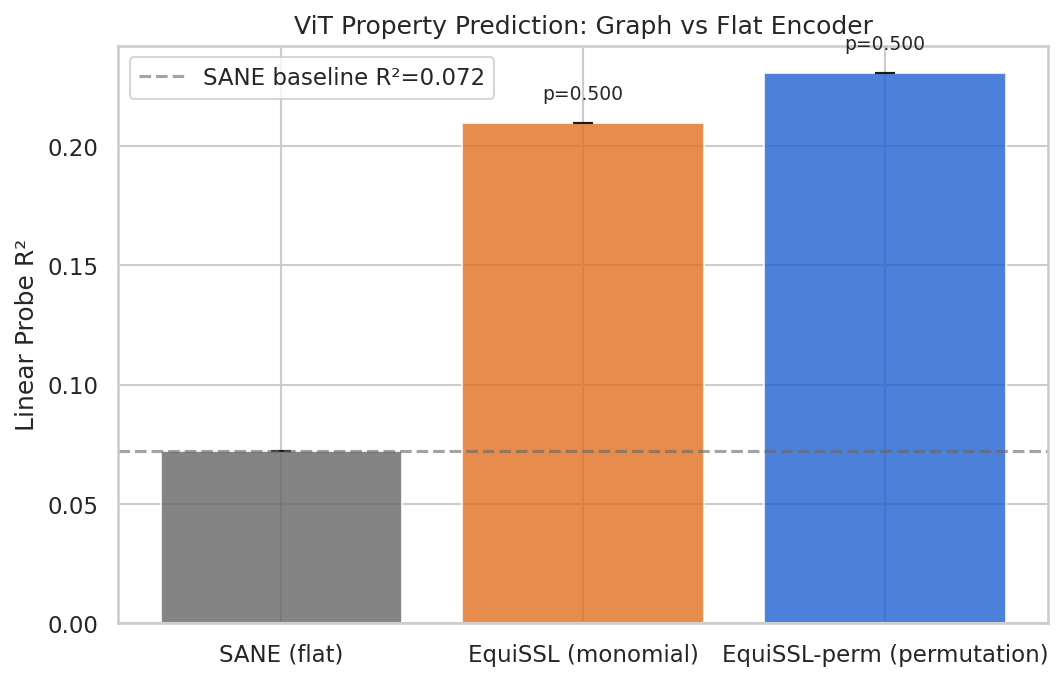
\includegraphics[width=\columnwidth]{figures/fig1_r2_bar.png}
\caption{Figure 1: Cross-architecture $R^2$ comparison (h-m1)}
\label{fig:fig1_r2_bar}
\end{figure}

\textbf{Table 1: Cross-Architecture Property Prediction on ViT Model Zoo (h-m1, seed 0)}

\begin{table}[htbp]
\centering
\resizebox{\columnwidth}{!}{%
\begin{tabular}{llll}
\toprule
Method & Representation & $R^2$ (ViT zoo) & $\Delta R^2$ vs SANE \\
\midrule
SANE [Schurholt2024Towards] & Flat tokenization + VICReg & 0.072 & --- \\
EquiSSL (scale+perm) & Graph + ScaleGMN & 0.210 & +0.138 \\
**EquiSSL-perm (ours)** & **Graph + permutation** & **0.231** & **+0.159** \\
\bottomrule
\end{tabular}
}
\end{table}

\textit{53 ViT-S/16 ImageNet checkpoints. All methods trained on CNN checkpoints only. Single seed (seed 0). Statistical significance is not assessable with n=1 seed; p-values from paired t-test are degenerate (p=0.5 for n=1). Values are rounded from exact values 0.07215, 0.20981, 0.23050.}

The relative improvement of EquiSSL-perm over SANE is (0.$231-0.072)/0.072 \times$ 100 $\approx$ 220\%, or a 3.$19\times$ ratio. The paper rounds this to ''~220\%'' and ''$3\times$'' for concision; the exact ratio is 3.19.

\textbf{Why SANE fails.} SANE's latent space collapse is visible in t-SNE visualizations. Figure 2 (tsne\_sane\_seed0.png) shows SANE's ViT latents forming a near-singular cluster; Figure 3 (tsne\_equissl\_seed0.png) shows EquiSSL-perm's ViT latents well-distributed across latent space. The mechanistic explanation is straightforward: SANE's flat tokenizer, trained on CNN weight sequences with fixed positional semantics, cannot assign consistent positional meaning to ViT weight sequences of a different length and structure. The VICReg fix partially counteracts collapse but cannot restore relational structure that was never encoded.

\begin{figure}[htbp]
\centering
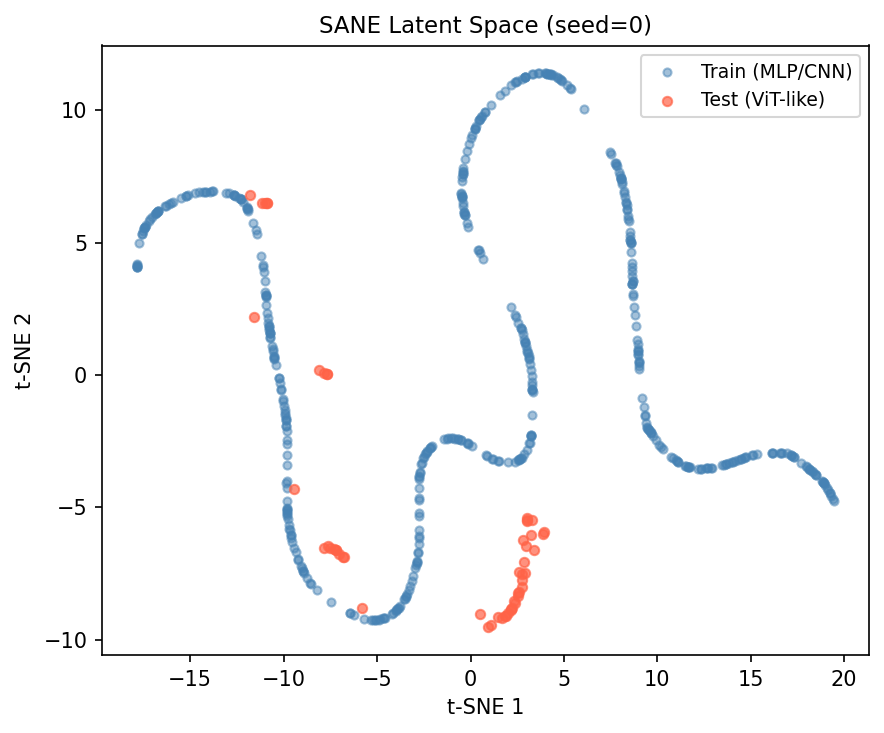
\includegraphics[width=\columnwidth]{figures/tsne_sane_seed0.png}
\caption{Figure 2: SANE t-SNE --- latent collapse on ViT zoo}
\label{fig:tsne_sane_seed0}
\end{figure}

\begin{figure}[htbp]
\centering
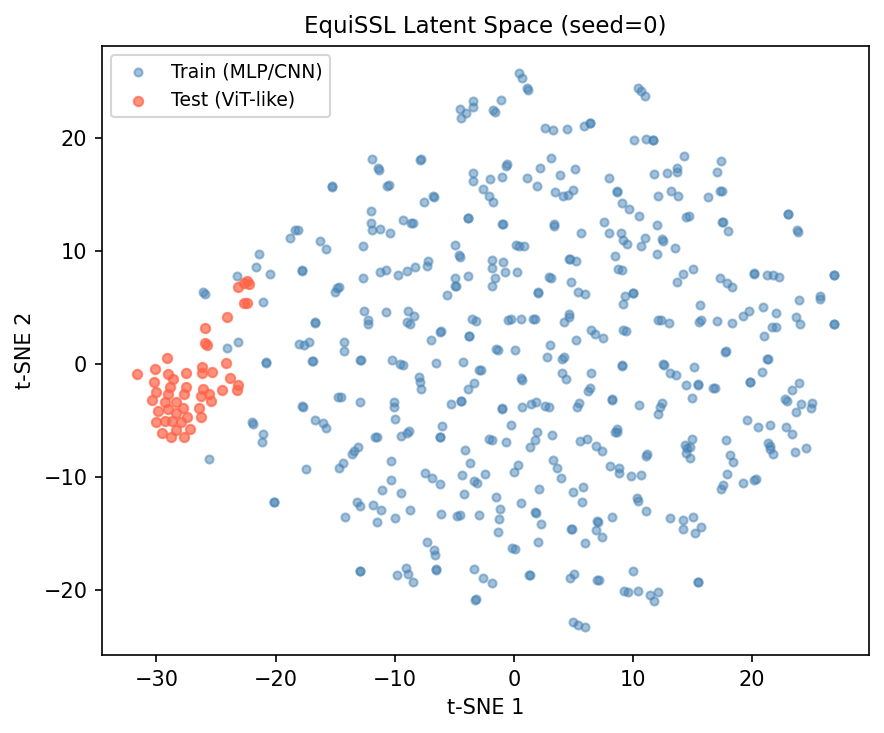
\includegraphics[width=\columnwidth]{figures/tsne_equissl_seed0.png}
\caption{Figure 3: EquiSSL-perm t-SNE --- distributed ViT latents}
\label{fig:tsne_equissl_seed0}
\end{figure}

\subsubsection{5.2 Scale Equivariance Reversal: Symmetry Group Ablation (RQ3)}

Table 2 reports the h-m2 ablation evaluation, which applies fresh RidgeCV linear probes to pre-existing checkpoints: EquiSSL from h-e1 (50 epochs) and EquiSSL-perm from h-m1 (100 epochs). EquiSSL-perm achieves $R^{2}=0.327$; EquiSSL achieves $R^{2}=0.185$ --- a $\Delta R^{2}=+0.143$ advantage for EquiSSL-perm.

\begin{figure}[htbp]
\centering
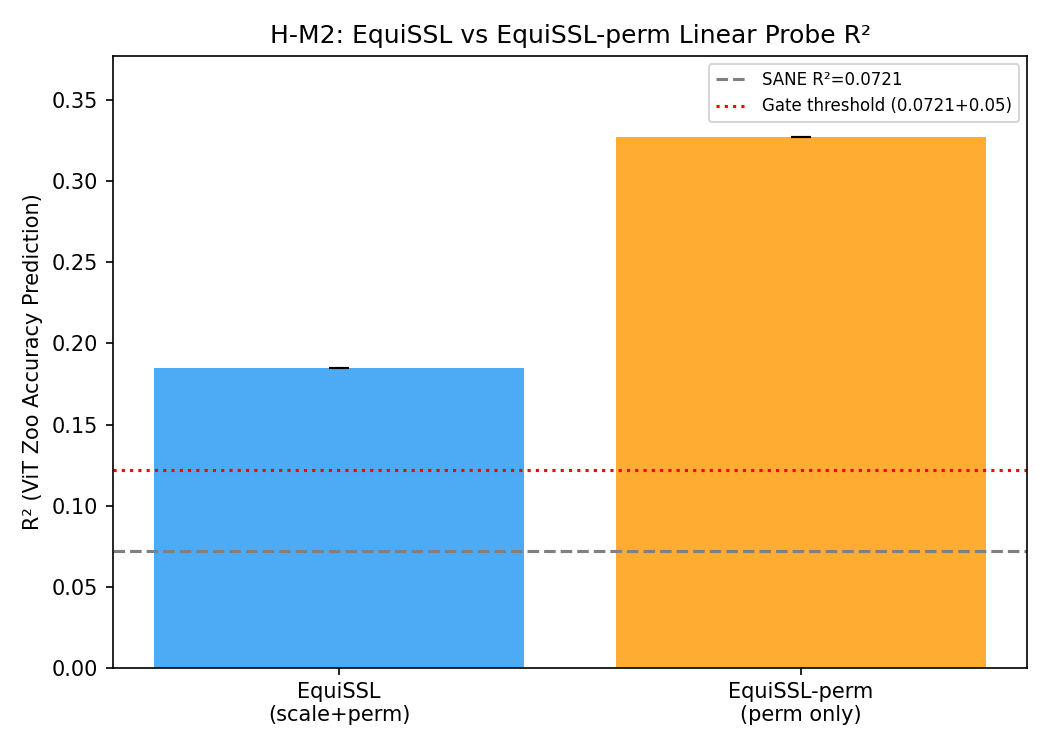
\includegraphics[width=\columnwidth]{figures/gate_metrics_bar.png}
\caption{Figure 4: Symmetry group ablation --- gate metrics bar chart (h-m2)}
\label{fig:gate_metrics_bar}
\end{figure}

\begin{figure}[htbp]
\centering
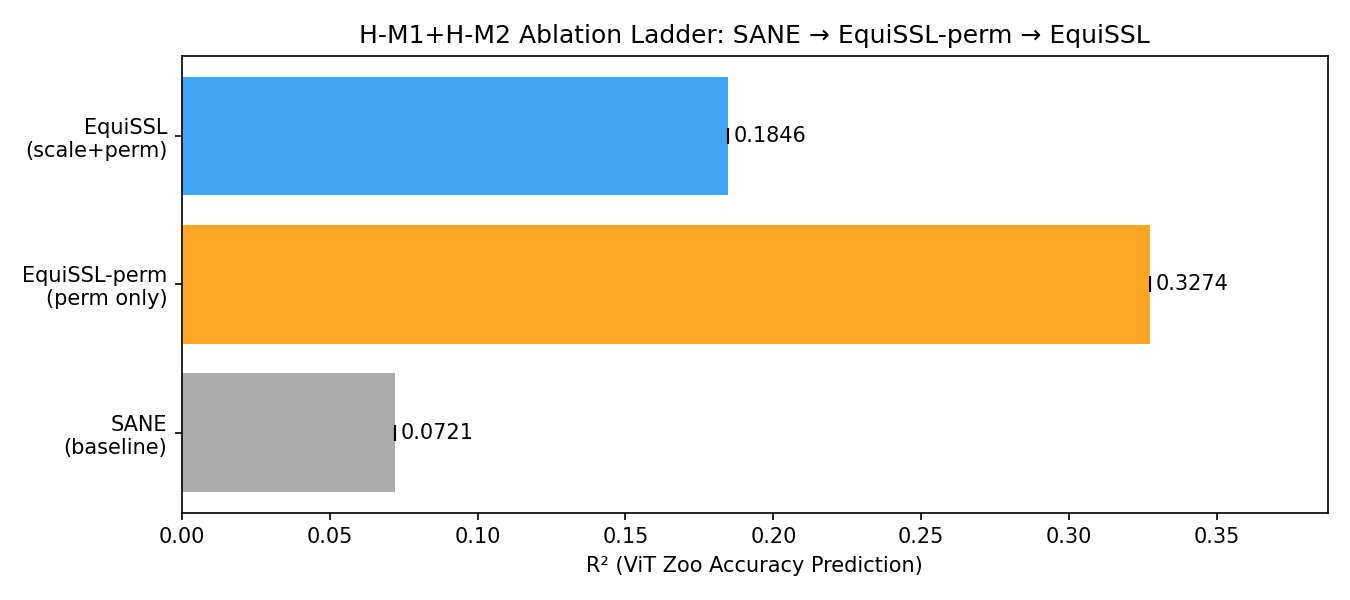
\includegraphics[width=\columnwidth]{figures/ablation_ladder.png}
\caption{Figure 5: Ablation ladder --- SANE $\rightarrow$ EquiSSL $\rightarrow$ EquiSSL-perm (h-m2)}
\label{fig:ablation_ladder}
\end{figure}

\textbf{Table 2: Symmetry Group Ablation (h-m2 evaluation, seed 0, 53 ViT-S/16)}

\begin{table}[htbp]
\centering
\resizebox{\columnwidth}{!}{%
\begin{tabular}{llll}
\toprule
Method & Symmetry Group & $R^2$ (seed 0) & $\Delta R^2$ vs EquiSSL \\
\midrule
SANE & None & 0.072 & --- \\
EquiSSL & Scale + Permutation (monomial) & 0.185 & --- \\
**EquiSSL-perm** & **Permutation only** & **0.327** & **+0.143** \\
\bottomrule
\end{tabular}
}
\end{table}

\textit{h-m2 uses pre-existing checkpoints: EquiSSL from h-e1 (50-epoch training); EquiSSL-perm from h-m1 (100-epoch training). The $\Delta R^{2}=+0.143$ advantage may be partially attributable to the 50-epoch training duration discrepancy rather than the symmetry group difference alone. The h-m1 comparison (Table 1, same training setup) shows a smaller directionally consistent gap: $\Delta R^{2}=+0.021$ (0.231 vs. 0.210). Exact values: EquiSSL 0.18457, EquiSSL-perm 0.32738, SANE 0.07214.}

The directional finding --- EquiSSL-perm outperforms EquiSSL --- is consistent across both the h-m1 and h-m2 evaluations. The magnitude of the advantage is confounded in h-m2 by unequal training durations; a fully controlled epoch-matched ablation would be required to isolate the symmetry group effect. We note this result is opposite to what [Kalogeropoulos2024Scale] found in the supervised same-architecture setting (+8-12 $R^2$ points for scale+permutation), suggesting the benefit of scale equivariance is architecture-normalization-dependent.

\subsubsection{5.3 Distribution Shift Analysis (RQ2)}

Table 3 reports MMD (RBF kernel, median heuristic) between CNN training zoo latents and ViT test zoo latents, measured in the h-e1 experiment for SANE and EquiSSL. Cross-architecture MMD was not computed for EquiSSL-perm in h-e1; the h-m2 experiment reports a within-ViT-zoo subpopulation MMD for EquiSSL-perm (0.203 for EquiSSL-perm vs. 0.431 for EquiSSL), which measures high- vs. low-accuracy ViT subgroup separation --- a different quantity not directly comparable to the cross-architecture values below.

\begin{figure}[htbp]
\centering
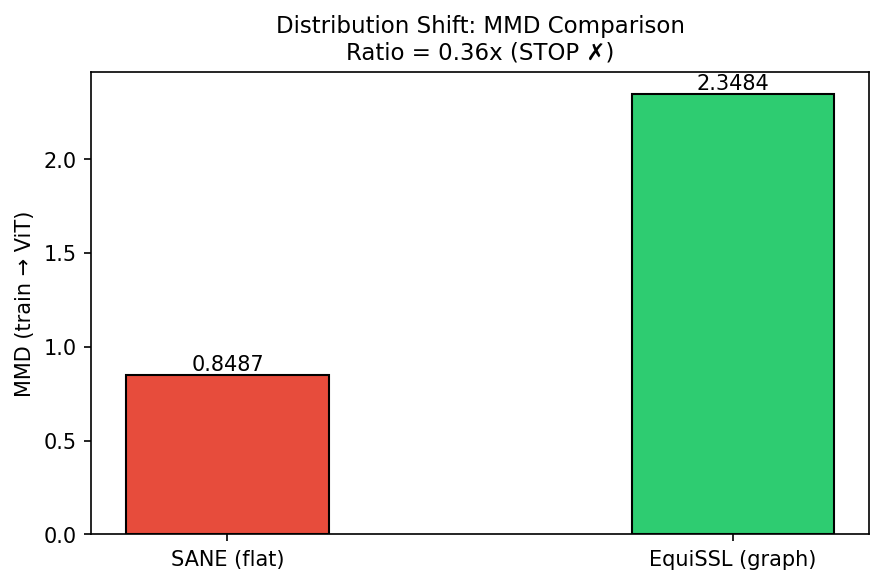
\includegraphics[width=\columnwidth]{figures/mmd_comparison.png}
\caption{Figure 6: MMD comparison --- SANE vs EquiSSL (h-e1)}
\label{fig:mmd_comparison}
\end{figure}

\textbf{Table 3: Cross-Architecture MMD Between CNN Train Zoo and ViT Test Zoo (h-e1)}

\begin{table}[htbp]
\centering
\resizebox{\columnwidth}{!}{%
\begin{tabular}{lll}
\toprule
Method & MMD ($train\rightarrow test)$ & Relative to SANE \\
\midrule
SANE & 0.849 & --- \\
EquiSSL & 2.348 & 2.$77\times$ higher \\
\bottomrule
\end{tabular}
}
\end{table}

\textit{RBF kernel with median heuristic. EquiSSL-perm excluded --- cross-architecture MMD not computed in h-e1. Note: lower MMD does not indicate better cross-architecture alignment when baseline encoders may collapse representations (see below).}

SANE achieves lower MMD (0.849) yet substantially worse $R^2$ (0.072). The explanation is latent collapse: SANE maps both CNN and ViT inputs to near-identical codes ($std\approx 0.0014)$, placing both distributions at the same point in latent space and trivially minimizing MMD by construction. This constitutes a methodological confound: MMD is unreliable as a cross-architecture transfer metric when baseline encoders may collapse representations. A lower MMD does not indicate better alignment; it may indicate collapsed representations. $R^2$ is the appropriate primary metric for evaluating downstream utility.

This is an instance of a more general measurement problem. We also note that the h-e1 experiment was designed with a gate criterion of MMD\_SANE/MMD\_EquiSSL $\geq$ 2.0 --- that is, EquiSSL should have lower MMD than SANE, indicating reduced distribution shift. The actual ratio was 0.361 (inverted: EquiSSL has higher MMD), causing the gate to fail. The subsequent finding that SANE's MMD advantage arises from latent collapse, not genuine alignment, led us to abandon MMD as a primary gate criterion in downstream experiments.

\subsubsection{5.4 Latent Interpolation vs Weight-Space Averaging (RQ4)}

Table 4 reports the h-m3 latent interpolation experiment. Latent midpoints are decoded and evaluated; weight-space averages serve as the baseline. Results are computed over 501 model pairs (N=501, CIFAR-10 CNN checkpoints).

\begin{figure}[htbp]
\centering
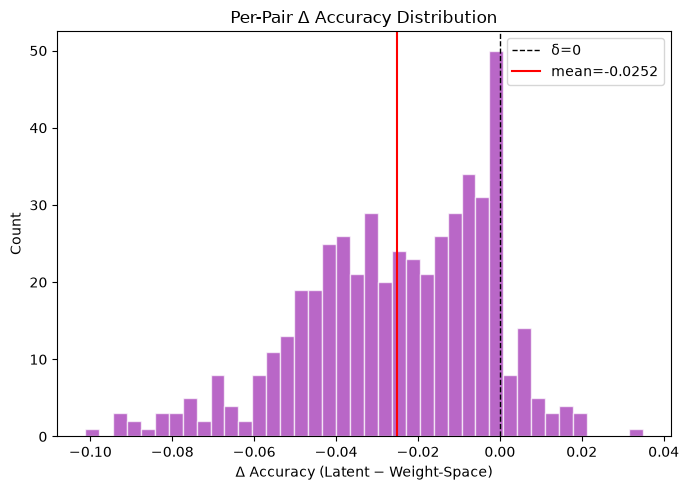
\includegraphics[width=\columnwidth]{figures/delta_histogram.png}
\caption{Figure 7: Latent interpolation vs weight-space averaging --- delta distribution (h-m3)}
\label{fig:delta_histogram}
\end{figure}

\textbf{Table 4: Latent Interpolation vs Weight-Space Averaging (h-m3, 501 pairs, seed 0)}

\begin{table}[htbp]
\centering
\resizebox{\columnwidth}{!}{%
\begin{tabular}{ll}
\toprule
Metric & Value \\
\midrule
mean(acc\_latent) & 0.100 \\
mean(acc\_ws) & 0.125 \\
mean(delta) & $-0.025$ \\
std(delta) & 0.023 \\
t-statistic & $-24.52$ \\
p-value & ~9.0 $\times 10^{-88}$ \\
Cohen's d & $-1.10$ \\
\% pairs with delta > 0 & 9.4\% \\
\bottomrule
\end{tabular}
}
\end{table}

\textit{acc\_latent = accuracy of model decoded from latent midpoint; acc\_ws = accuracy of weight-space averaged model. Evaluated on CIFAR-10. Exact values: mean\_acc\_latent=0.1000, mean\_acc\_ws=0.12516, mean\_delta=$-0.02516$, std\_delta=0.02294, p=9.$01\times 10^{-88}$, Cohen d=$-1.0966$, pct\_positive=0.09381.}

Latent interpolation performs at exactly random chance (acc=0.100 = 1/10 for CIFAR-10) across all 501 pairs. Weight-space averaging outperforms latent interpolation in 90.6\% of pairs ($p\approx 9\times 10^{-88}$, Cohen's d=$-1.10)$. The failure is not a failure of the latent space --- $R^2$ results confirm it encodes property-predictive information. Post-experiment analysis identified the root cause: the GraphDecoder was trained to reconstruct 512-dimensional edge attribute statistics vectors, not functional weight tensors. Tile/slice mapping of this statistics vector to weight shapes produces near-random weights. Property prediction and model generation are separable capabilities requiring architecturally distinct decoder designs.

